%% LaTeX2e class for seminar theses
%% sections/content.tex
%% 
%% Karlsruhe Institute of Technology
%% Institute for Program Structures and Data Organization
%% Chair for Software Design and Quality (SDQ)
%%
%% Dr.-Ing. Erik Burger
%% burger@kit.edu
%%
%% Version 1.0.2, 2020-05-07

\section{Technische  Funktionsweise der C2C-Kommunikation}
\label{ch:FirstContentSection}

%% -------------------
%% | Example content |
%% -------------------
Im folgenden Abschnitt wird die Funktionsweise der C2C-Kommunikation und die dafür benötigte Infrastruktur näher beschrieben. Der Nachrichtenaustausch zwischen Fahrzeugen beruht auf Public-Key Kryptografie, somit werden die Nachrichten mit einer Signatur und einem Zertifikat versehen, die von einer zentralen Stelle ausgegeben werden. Weiterhin wird auf die Nachrichtenformate der C2C-Kommunikation eingegangen, sowie auf die darin gespeicherten Daten, die möglicherweise für die Identifikation des Fahrzeugs benutzt werden können. Des Weiteren werden mögliche Angriffe auf die Pseudonymität der Nachrichten aufgeführt, aufgrund deren Bewegungsprofile von Fahrzeugen erstellt werden können.

\subsection{Public-Key Infrastruktur}
\label{sec:FirstContentSection:FirstSubSection}
 
Um den oben genannten Nachrichtenaustausch zu ermöglichen, braucht man eine entsprechende Public-Key Infrastruktur (PKI), die aus einer oder mehreren Certification Authorities (CAs) besteht. Die CAs sind in der Lage, digitale Zertifikate zu erstellen, diese Zertifikate der End-Entitäten zu erteilen und zu verifizieren. Als End-Entitäten fungieren ITS-Stationen (u.a. Fahrzeuge), die die erstellten Zertifikate für die Kommunikation untereinander verwenden und somit die Authentizität von einer Nachricht beweisen und überprüfen können  \cite{Strubbe2017}. 

Die PKI wird aus drei Stufen zusammengesetzt \cite{SecurityCITS}: 
\begin{itemize}
	\item Root-CAs (erstellen Zertifikate für untergeordnete CAs)
	\item Mindestens zwei Sub-CAs
	\item End-Entitäten (EEs)
\end{itemize}

Darüber hinaus gibt es zwei Arten von Sub-CAs: Enrolment Authorities (EA) und Authorization Authorities (AA). Die EAs erstellen langlebige Zertifikate für EEs, die für die Authentifizierung innerhalb der PKI verwendet werden. Die AAs hingegen stellen kurzzeitige Zertifikate zur Verfügung, mit denen die EEs (z.B. Fahrzeuge) untereinander kommunizieren können ohne die Pseudonymität von einzelnen Entitäten zu verletzen. Der schematische Aufbau von einer PKI wird in der Abbildung \ref{fig:pki} verdeutlicht.

\begin{figure}
	\centering
	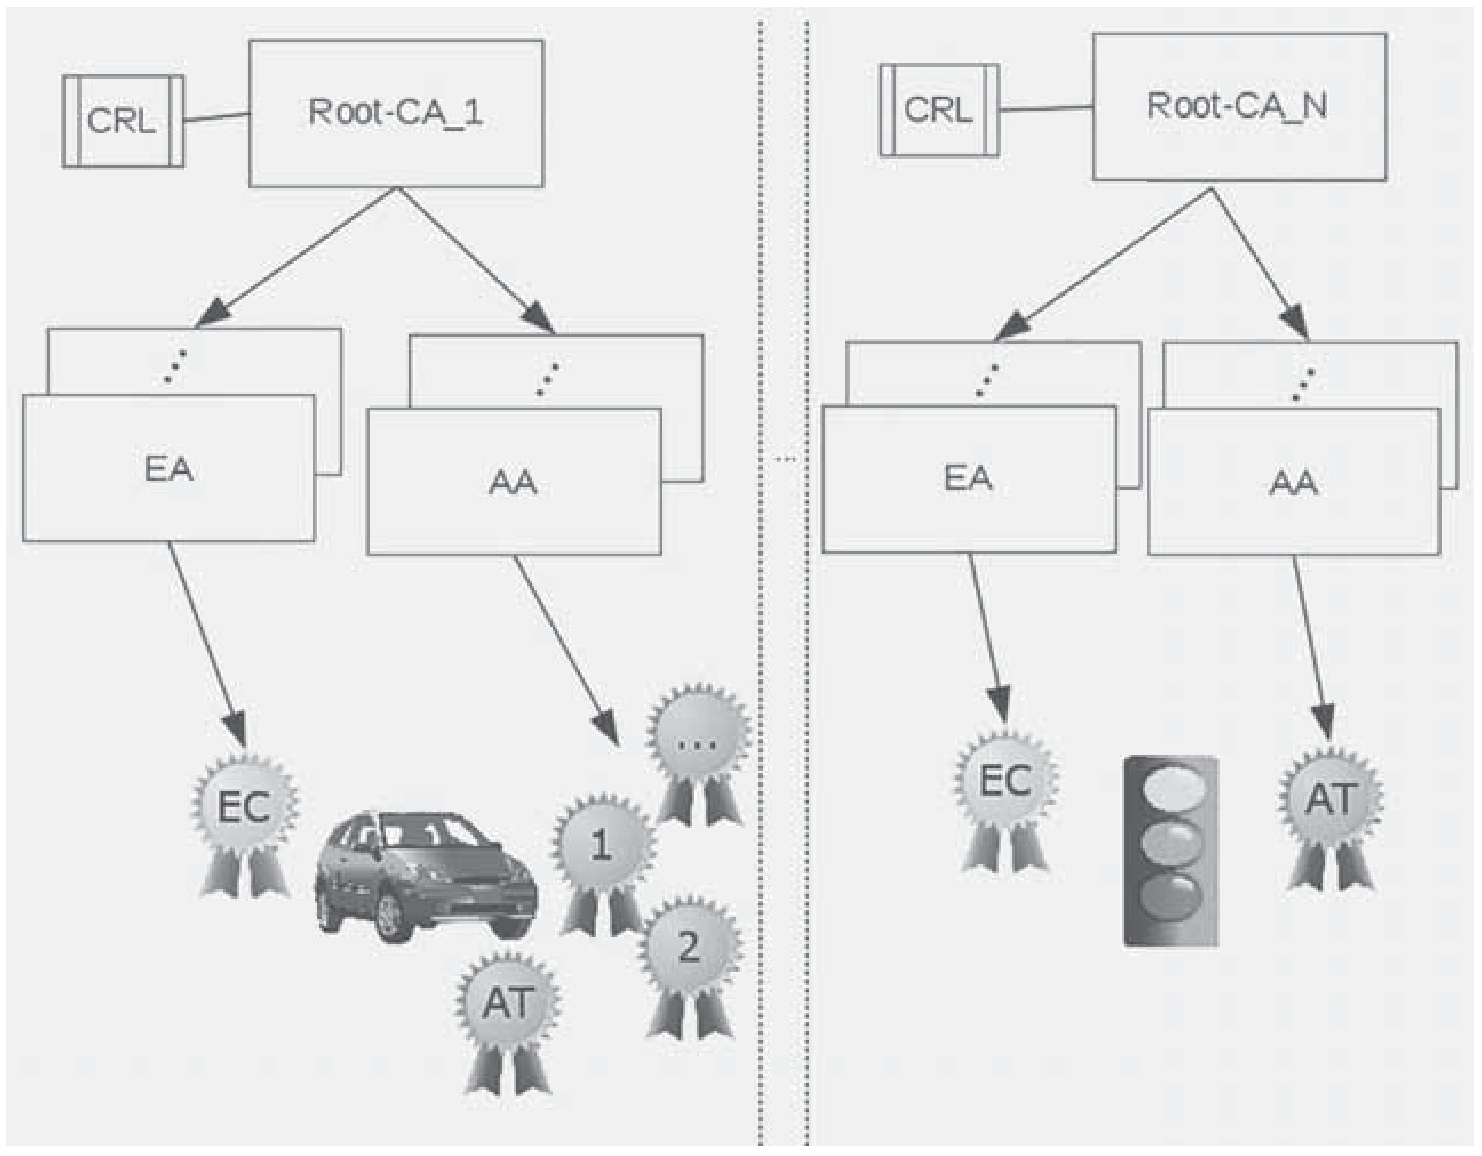
\includegraphics[width=0.7\linewidth]{images/PKI}
	\caption{Aufbau einer PKI für C2X Kommunikation nach \cite{Strubbe2017}}
	\label{fig:pki}
\end{figure}

Bevor jegliche Kommunikation stattgefunden hat, muss sich die End-Entität zunächst bei der zugehörigen EA registrieren und ein Enrolment Credential erhalten, das mehrere Jahre gültig ist. Die EA bekommt dabei die Registrierungsinformationen von der EE, zum Beispiel ihre Fahrzeugidentifizierungsnummer und ihren öffentlichen Schlüssel. Die EE signiert den initialen Zertifikatsrequest mit ihrem eingebauten privaten Schlüssel und übermittelt ihn an die EA. Falls die Daten übereinstimmen, erhält die EE einen Enrolment Credential (EC).

Mit einem gültigen EC kann die EE weiterhin sogenannte Authorization Tickets (AT) bei der AA beantragen. ATs sind kurzzeitgültige Zertifikate für C2X Kommunikation, die oft gewechselt werden und somit der Senderpseudonymität dienen. Die Nachrichten sollten keinen eindeutigen Identifikator erhalten, damit kein Personenbezug hergestellt werden kann. Daher werden CAMs und DENMs mit ATs signiert und nicht mit den langlebigen ETs, die für eine EE über mehrere Jahre gültig ist. 

Ein AT wird von einer Entität bei der AA beantragt. Die Anfrage an die AA enthält unter anderem verschlüsselte Daten, die nur von der entsprechenden EA ausgelesen werden können \cite{ETSI2018}, darunter die EC von der Entität. Die EA bestätigt die Authentizität der Daten mit dem angehängten EC und schickt eine Statusmeldung an die AA, ohne diese zusätzliche Information preiszugeben. Es ist wichtig, die EA und AA organisatorisch getrennt zu halten, da sonst bei der AT-Anfrage eine Zuordnung zu der End-Entität bzw. ihrem EC möglich wäre.


Nachdem die mit dem AT signierte Nachricht erfolgreich an die empfangende EE übermittelt wurde, nutzt sie den AT um die Nachricht zu verifizieren. Dies erfolgt mittels einer Kettenprüfung durch die AA und das entsprechende Root-Zertifikat, wodurch die Authentizität der Nachricht festgestellt wird.

In Europa ist zusätzlich zu der oben beschriebenen PKI eine globale Vertrauensliste vorgesehen, die innerhalb der europäischen Grenzen alle vertrauenswürdige Root-CA-Zertifikate beinhaltet. Diese wird von einem zentralen Trust List Manager (TLM) erstellt und elektronisch signiert. Somit wird die Interoperabilität von europäischen PKIs über Grenzen sichergestellt. Darüber hinaus ist es wichtig, die nicht mehr vertrauenswürdigen Zertifikate zurückziehen zu können - dies wird durch sogenannte Certificate Revocation Lists (CRL) sichergestellt. Diese werden allen PKI-Teilnehmern von der jeweiligen Root-CA zur Verfügung gestellt und enthalten die Liste mit allen revozierten Zertifikaten.  

\subsection{Nachrichtenformate}
\label{sec:FirstContentSection:SecondSubSection}

Die Nachrichtenformate, die für die oben beschriebene PKI nötig sind, wurden von dem Europäischen Institut für Telekommunikationsnormen (ETSI) definiert. Im Weiteren wird auf \cite{ETSI2018} verwiesen, in dem die Paketstruktur für gesicherte C2X-Nachrichten und deren Zertifikatsformat festgelegt wurde. 

Der grobe Aufbau einer gesicherten C2X-Nachricht wird in der Abbildung \ref{fig:nachrichtenaufbau} dargestellt. Sie enthält unter anderem die ECDSA-Signatur (\cite{Barker2013}), den Verifikationsschlüssel des Senders und die eigentliche Nachricht, die im Payload gespeichert ist. Für die Car-2-Car Kommunikation sind zurzeit zwei Nachrichtenformate vorgesehen:
\begin{itemize}
	\item die Cooperative Awareness Message (CAM) und die 
	\item Decentralized Environmental Notification Message (DENM) \cite{ETSI2013}.
\end{itemize}

\begin{figure}
	\centering
	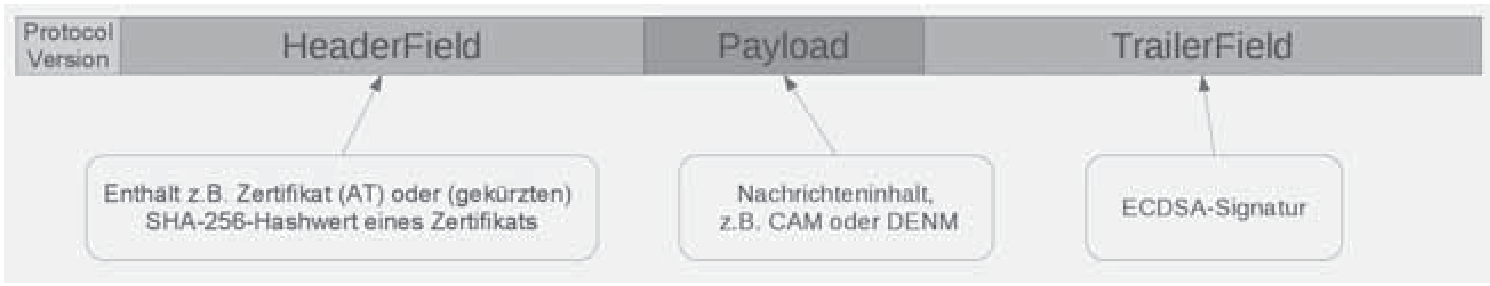
\includegraphics[width=0.7\linewidth]{images/Nachrichtenaufbau}
	\caption{Grobaufbau einer verschlüsselten Nachricht nach \cite{Strubbe2017}}
	\label{fig:nachrichtenaufbau}
\end{figure}

Im Weiteren wird nur die CAM betrachtet, da die DENM keine personenbezogenen Daten beinhaltet und im datenschutzrechtlichem Sinne kein Problem darstellt \cite{Kiometzis2017}. Der Aufbau einer CAM wird in der Abbildung \ref{fig:cam} dargestellt. Sie besteht aus vier Elementen: Header, CAM Information, Signature und Certificate. Die tatsächliche Information über das Fahrzeug wird im Block CAM Information gespeichert. Er beinhaltet sowohl dynamische Daten (z.B. Last Geographic Position, Speed) als auch statische Daten über das Fahrzeug, die trotz ständigem Pseudonymwechsel identisch bleiben (z.B. Length, Weights). Eine CAM erhält keinen primären Identifikator, aufgrund dessen eine eindeutige Zuordnung zum Fahrzeug möglich wäre.

\begin{figure}
	\centering
	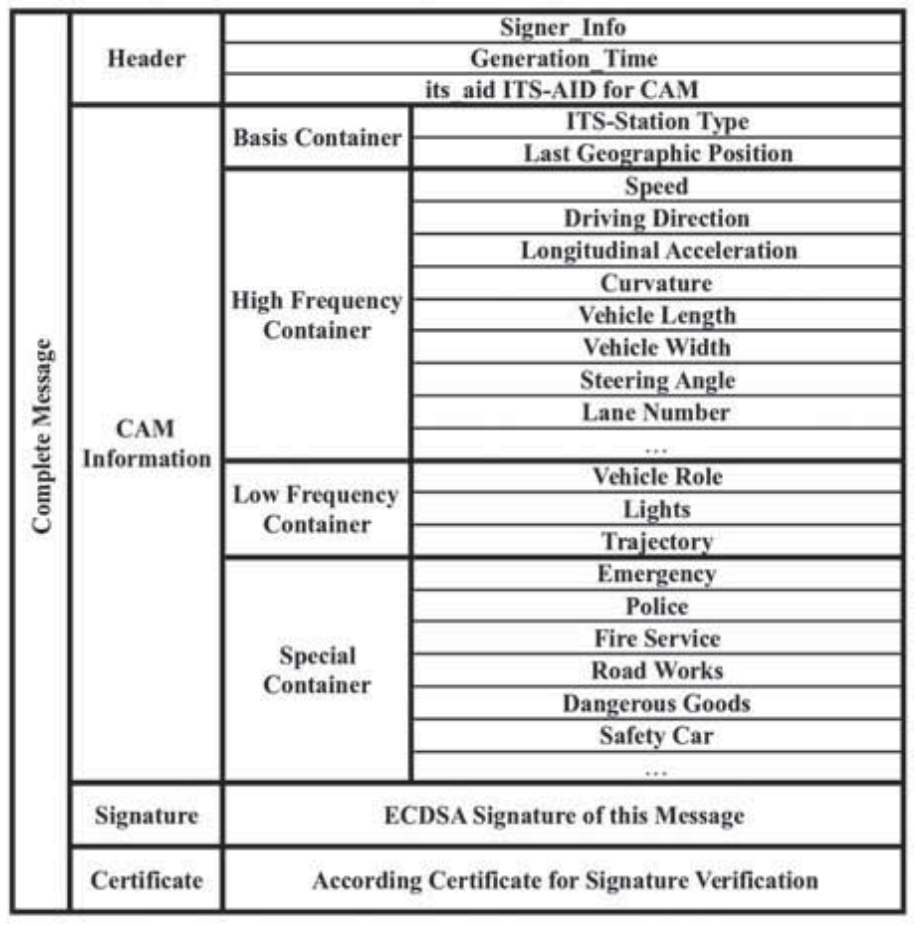
\includegraphics[width=0.4\linewidth]{images/CAM}
	\caption{Detallierter Aufbau einer CAM nach \cite{Kiometzis2017}}
	\label{fig:cam}
\end{figure}

\subsection{Angriffsmöglichkeiten}
\label{sec:FirstContentSection:ThirdSubSection}

Auch wenn CAMs keine primären Identifikationsmerkmale erhalten, existieren es mehrere Möglichkeiten, um mithilfe von CAMs Bewegungsprofile von Fahrzeugen zu erstellen. Dies kann zu diversen Risiken für die Privatsphäre führen, falls der Personenbezug von Fahrdaten hergestellt werden kann. Im folgenden Abschnitt werden einige Angriffsarten auf die Pseudonymität von CAMs näher beschrieben und analysiert. 

Als erstes Beispiel sei ein sogenannter 'Big Brother Angreifer' angeführt, der eine Infrastruktur von Empfangseinrichtungen in einer geografischen Region betreibt und in der Lage ist, in dieser Gegend CAMs von Fahrzeugen zu erfassen und auszuwerten. Das wäre möglich, indem der Angreifer zum Beispiel eine Fahrzeug-Flotte aufstellt, die eingehende CAMs an einen zentralen Server übermittelt. Auch wenn vorbeifahrende Fahrzeuge ihr Pseudonym jede 10 Sekunden ändern würden, könnten sie mit solch einer Infrastruktur verfolgt werden \cite{Wiedersheim2010}. Da diese Art von Überwachung alle Fahrzeugdaten in der Gegend erfassen würde, könnte sie für breitere Verkehrsanalysen genutzt werden.
 
Darüber hinaus gibt es einige Möglichkeiten, die Bewegungen von einzelnen Fahrzeugen detailliert aufzuzeichnen. Zum Beispiel kann man mithilfe eines an das Fahrzeug befestigtes Überwachungstools sogenannte CAM-Traces erstellen, d.h. die gefahrene Strecke eines Fahrzeugs und alle von ihm auf dieser Strecke erstellten CAMs. Auch wenn das Fahrzeug regelmäßig seinen Signaturschlüssel wechselt, würde es reichen, nur eine CAM aus der CAM-Trace dem Fahrzeug eindeutig zuzuordnen, um die gesamte CAM-Trace diesem Fahrzeug zuzuordnen \cite{Kiometzis2017}. 

Es existiert eine Reihe von Methoden, um diese Zuordnung durchzuführen. In \cite{Ullmann2016} wurde dargelegt, dass sie aufgrund der sog. Secondary Vehicle Identifier erfolgen kann. Diese wird von diversen drahtlosen Schnittstellen im Auto zur Verfügung gestellt (z.B. eine Headunit, die eine öffentliche Bluetooth-Schnittstelle mit einem nutzerfreundlichen Namen besitzt). Die Secondary Vehicle Identifiers sind einfach zu erfassen und können einer eindeutigen Zuordnung der empfangenen CAM-Trace zum Fahrzeug dienen. 





\section{Vereinbarkeit mit datenschutzrechtlichen Prinzipien}
\label{ch:SecondContentSection}

Die Datenschutzgrundverordnung (DSGVO) ist eine Verordnung, mit der die Regeln zur Verarbeitung personenbezogener Daten in der Europäischen Union vereinheitlicht werden. Sie ist am 25. Mai 2018 inkraft getreten und hat zu dem Zeitpunkt geltende Richtlinie 95/46/EG zum Schutz natürlicher Personen bei der Verarbeitung personenbezogener Daten und zum freien Datenverkehr ersetzt. 

In diesem Abschnitt wird diskutiert, ob die Erhebung von Fahrdaten in einer PKI ein datenschutzrechtliches Problem darstellt, und geprüft, ob die DSGVO in diesem Fall anwendbar ist. Dafür werden einige Verfahren vorgestellt, mithilfe von denen ein Bewegungsprofil und deren Personenbezug aus den Fahrdaten hergestellt werden kann. Darüber hinaus 

Warum stellen IVS ein datenschutzrechtliches Problem dar? Ist DSGVO anwendbar? 

(Beispiel von rechtlicher Probl	emstellung und Richtlinien zu deren Lösung - \cite{EUCooperativeV2X} ) - wird wahrscheinlich nicht behandelt oder kurz erwähnt, da wir uns auf DSGVO konzentrieren

\subsection{Anwendbarkeit der DSGVO}
\label{sec:SecondContentSection:SecondSubsection}

Zunächst wird die Anwendbarkeit der DSGVO auf die in CAMs erhaltene Fahrdaten diskutiert. Falls diese Daten personenbezogen sind, beziehungsweise für eine eindeutige Identifizierung der Person benutzt werden können, fällt ihre Verarbeitung unter DSGVO und somit sind sämtliche Grundsätze anwendbar, wie zum Beispiel Grundsatz der Datenminimierung und Grundsatz der Integrität und Vertraulichkeit. 

\subsubsection{Bewegungsprofile und Verhaltensprofile}
\label{sec:SecondContentSection:SecondSubsection:FirstSubSubsection}

Wie in Kapitel \ref{sec:FirstContentSection:ThirdSubSection} erwähnt, erhalten CAMs keine primären Identifikationsmerkmale, jedoch ist es möglich, mithilfe von einer geeigneten Infrastruktur Bewegungsprofile von Fahrzeugen zu erstellen. Außerdem enthalten CAMs statische Attribute wie zum Beispiel die Fahrzeuglänge und dessen Gewicht, die eine zusätzliche Kennzeichung von einem Fahrzeug erlauben. So wäre es unter Umständen möglich, ein bestimmtes Modell von einem bestimmten Hersteller nur aus der CAM zu erkennen. In wenig befahrenen Gebieten kann dies zu einer eindeutigen Identifizierung von dem Fahrzeug und einer Zuordnung zum ganzen CAM-Trace führen. Darüber hinaus kann man mithilfe von Secondary Vehicle Identifiers (z.B. einer öffentlich verfügbaren Bluetooth-Schnittstelle) diese Zuordnung durchführen. Letztens, da die CAM-Daten mit einer hohen Frequenz versendet werden, kann der Fahrweg mit einer hohen Zuverlässigkeit vorausberechnet und zurückberechnet werden. 

Somit ist es grundsätzlich möglich, aus einem flächendeckenden Datenbestand aus CAMs über einen längeren Zeitraum Bewegungsprofile zu erstellen, und somit gegebenenfalls auch Verhaltensprofile. In \cite{Dettki2005} wurde zum Beispiel nachgewiesen, dass anhand der Lenkbewegungen ruhige von nervösen Fahrer unterschieden werden können. Außerdem wäre es durch die Anwendung von künstlicher Intelligenz und maschinellem Lernen durchaus möglich, große Datenbestände von Bewegungsprofilen und somit die zugehörigen Fahrer zu klassifizieren, falls Personenbezug hergestellt werden kann. 

\subsubsection{Herstellbarkeit Personenbezug}
\label{sec:SecondContentSection:SecondSubsection:SecondSubSubsection}

Der Gegenstand von DSGVO sind personenbezogene Daten. Selbst wenn CAMs direkt keine primären Identifikationsmerkmale enthalten, kann deren Personenbezug grundsätzlich mit Zusatzwissen hergestellt werden. Technisch kann das durch eine Auflösung des Pseudonyms bei einem sogenannten Pseudonym Provider erfolgen \cite{Kiometzis2017}, aber auch durch andere Wege. Zum Beispiel, kann man anhand einer CAM-Trace aufgrund der am meisten gefahrenen Strecken den Wohn- und Arbeitsort einer Person identifizieren. Außerdem wäre es zum Beispiel möglich, durch Datenanalyse die Outliers in der Menge von den aufgezeichneten CAM-Traces identifizieren und versuchen, sie auf Personen mit entsprechendem Tagesablauf zurückzuführen. Besonders in wenig befahrenen Gebieten wäre diese Technik erfolgreich. Letztendlich wäre in vielen Situationen der einfachste Weg, vor Ort das Fahrzeug zu identifizieren (z.B. durch aufgezeichnete Videos oder Zeugenaussagen), und später aus dem Datenbestand die entsprechende CAM-Trace auszusuchen. Alle oben ausgeführten Techniken voraussetzen natürlich eine umfassende Erfassung von Fahrdaten und einen vorhandenen Bestand von Bewegungsprofilen (z.B. den in Kapitel \ref{sec:FirstContentSection:ThirdSubSection} beschriebenen Big Brother Angreifer).

Eine besondere Sensibilität allein aus der Art der Daten wird nach Art. 9 EU-DSGVO nicht begründet \cite{Weichert2016}.

\cite{Weichert2016} - Datenschutzrechtliche Analyse der Car-2-Car-Communication, guter Ausgangspunkt.

\subsection{Grundsatz der Datenminimierung}

Art.5 Abs.1c DSGVO - "Datenminimierung". 

Geeignete Pseudonymisierung

\subsection{Recht auf Datenübertragbarkeit}

Art.20 DSGVO - "Recht auf Datenübertragbarkeit"

\cite{Straub2018} - Analyse der Datenübertragbarkeit, Begründung der DSGVO-Anwendbarkeit

\subsection{Datenschutzmaßnahmen}
Das schutzwürdige Interesse an der Vermeidung von Bewegungsprofilen besteht in jedem Fall; eine individualisierte Zweitnutzung setzt deshalb eine explizite Einwilligung voraus. (zweitnutzung - begehrlichkeit!)- \cite{Weichert2016}

\cite{Seewald2018} - alle o.g. Datenschutzmaßnahmen + "obligation to report a data breach, to conduct a data protection impact assessment". "analytical progress of AI". Guter Ausgangspunkt für Kapitel \ref{sec:SecondContentSection:SecondSubsection}

Die in \cite{Kiometzis2017} aufgeführten Empfehlungen untersuchen und analysieren. 

%Add additional content sections if required by adding new .tex files in the
%\code{sections/} directory and adding an appropriate 
%\code{\textbackslash input} statement in \code{thesis.tex}. 
%%% ---------------------
%% | / Example content |
%% ---------------------